\chapter{Verification}
\label{verification}

This section describes the verification activities undertaken as part of this project, giving examples of how they were applied to each of the modules in the design. Firstly, the use of the V-model process for verification in this project is discussed. This is followed by a discussion of how verification methodologies were utilised throughout verification, simulation and testing in this project. The verification plan, which maps directly to the original project requirements, is presented. The verification results are then presented. The verification of each module in the system architecture is discussed with example simulation and verification results. 

In the interest of maintaining clarity of terminology used in this context, terms will be explained. In this section, verification will refer to the direct mapping and confirmation of functionality to the requirements of the system. Simulation will comprise of the analysis of produced waveforms. Testing will cover activities that incorporating timings to ensure the correct physical behaviour of the design. The term Modules will be used to refer to the high level system modules in the system architecture. There are four modules in the design: Input Processing, PWM Regulation, ADC and Motor Driving. Sub-modules will be used to refer to any design unit used within the high-level module. These sub-modules directly map to an individual requirement whereas the modules refer to a group of requirements.

\section{Verification Stages}

The V-model, shown in Figure \ref{V-model}, encourages verification of every level of the design. The verification stages follow a bottom-up methodology with a complimentary verification stage for each design activity. The first stage involves post-layout simulation to check the conformity of the design to the design rules set by the FPGA. This activity is performed automatically by the Lattice Diamond tool-suite. Following this, individual modules are verified. This stage benefits from small contained modules with a single testable functionality. After the modules have been verified, the integration of and interactions between the modules can be verified. This process can be repeated until all modules are integrated, at which point the complete design is verified. Direct validation of requirements is the final verification stage in the V-model. Each of the requirements of the design must be validated in order to produce a validated VHDL design.

Requirements at each phase must be directly testable in order to produce a validated design. During the design phases, a test plan was produced in order to verify the requirements of that phase. This includes behavioural verification which involves ensuring the outputs produced by the unit under test correspond correctly to the input sequence. Using VHDL, it is also possible to accurately model the timing behaviour. This makes it easier to verify the real-time behaviour required by motor control applications.

%In order to test analogue components, mixed-signal simulation tools can be used\cite{Acero}. 

\section{Verification Methodologies}

Verification methodologies were adopted to aid the automation of verification, simulation and testing in this project. Two methodologies, introduced in Section \ref{litreview}, were adopted in order to perform the required verification for this project: UVVM (Universal VHDL Verification Methodology)\cite{uvvmref} and OSVVM (Open Source VHDL Verification Methodology)\cite{osvvmref}. UVVM has been adopted in order to provide stimulus and value checking whereas OSVVM has been adopted to provide automatic coverage collection. The application of these methodologies is described below.

\subsection{Universal VHDL Verification Methodology}

UVVM was applied to the design for simulation stimulus, value checking and timing verification. A number of functions are provided by the methodology for analysing the values of signals at different points in a simulation which can be triggered by events or time-windows. This allows the behavioural response of the design to be verified alongside the timing of the response. As well as producing graphical simulation results which display the states of each signal in the unit under test (UUT), textual results can be produced to automate the checking of required values at different points in the simulation. The use of these functions allowed the functional and timing behaviour of the system modules to be verified.

Figure \ref{position_uvvm} shows the application of UVVM to an example design module, the Position Acquisition module. The diagram, generated by the VHDL editor Sigasi, shows how the inputs of a UUT can be stimulated and how its outputs are monitored by the UVVM process (labelled uvvm\_driver in the diagram). This is shown in Figure \ref{position_uvvm}. The diagram shows the input clock, reset and position buttons being provided to the left of the UUT by the UVVM driver. This process allowed each of the test cases to be applied to the UUT. The response of the calculated position, shown on the right of the UUT, was then compared to the expected position for each case. This methodology was used for each module in the design. Example UVVM code used to verify the Position module is shown in Appendix Item \ref{UVVM_Position_Code}.

\begin{figure}[h]
\centering
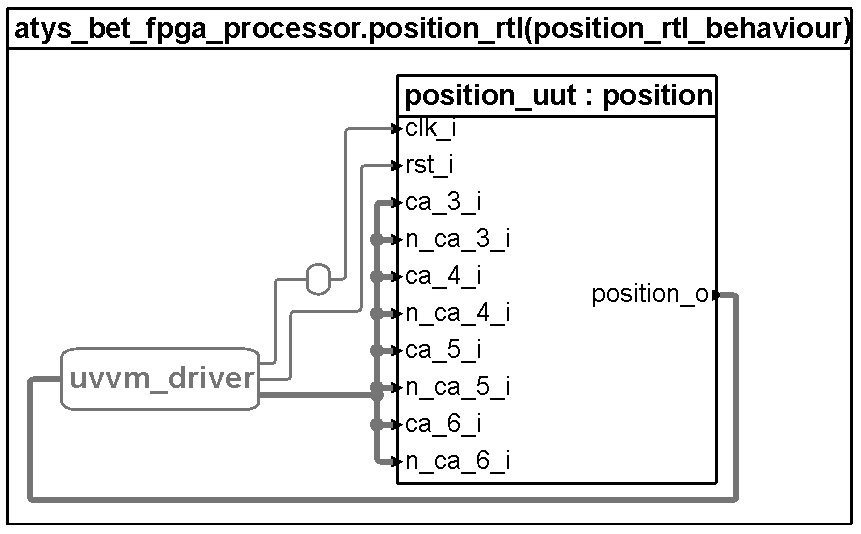
\includegraphics[width=0.75\textwidth]{images/uvvmblockdiagram.pdf}
\caption{UVVM simulation setup showing the input driving and output sensing for the Position Acquisition module of the ATyS design (diagram generated by Sigasi from the design code of the project)}
\label{position_uvvm}
\end{figure}



\subsection{Open Source VHDL Verification Methodology}

The application of OSVVM allowed for the 100\% coverage, required by SIL, to be proven automatically. Functional coverage was applied to the design to ensure that the test plan had been completed. By setting up transition bins, the states of the UUT were tracked throughout the simulations and a calculation of the coverage was performed by the OSVVM process. Example OSVVM code, showing the mapping of state machine transitions for the example UUT is shown in Appendix Item \ref{OSVVM_Motor_Bins}. The operation of this tracking can be seen in Figure \ref{osvvm_sim} where the OSVVM coverage process monitors the UUT throughout the simulation. This diagram, also generated using Sigasi, shows how the OSVVM process monitors the stimulus provided by the UVVM process as well as the states of the example UUT. This was applied to all state machines in the design to ensure that all valid states of the system were realised in the simulation process.

\begin{figure}[h]
\centering
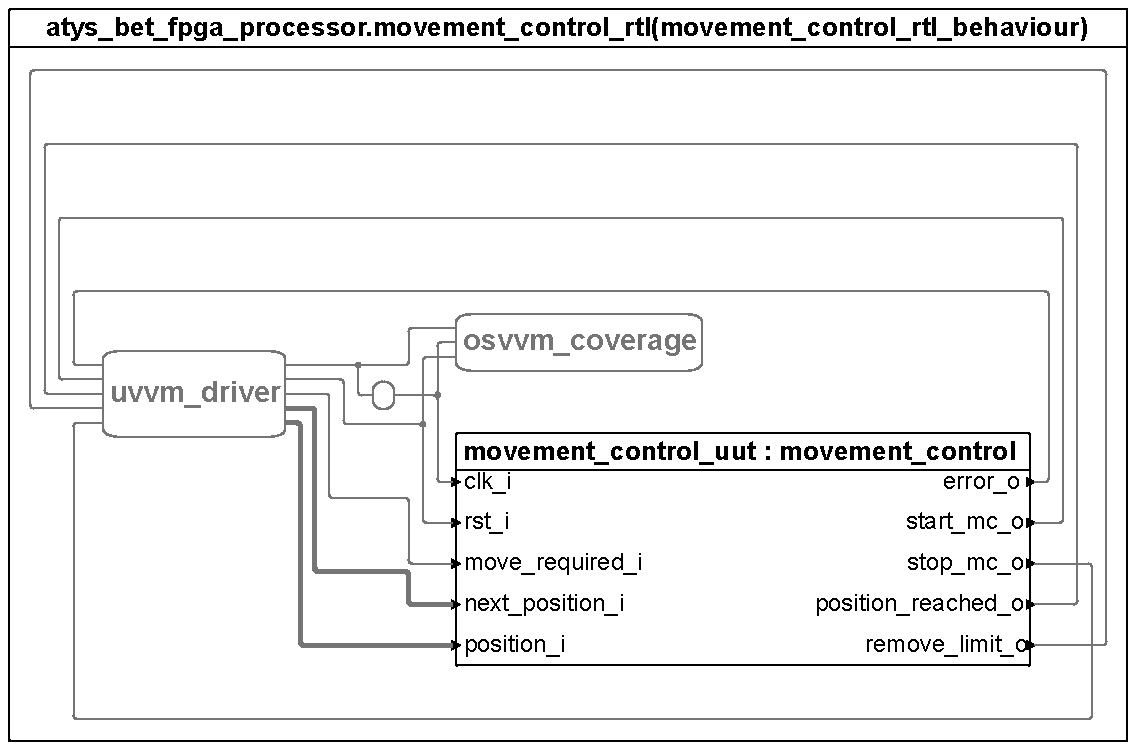
\includegraphics[width=\textwidth]{images/osvvmblockdiagram.pdf}
\caption{OSVVM process tracking the coverage on a UVVM driven simulation (diagram generated by Sigasi from the design code of the project)}
\label{osvvm_sim}
\end{figure}

\section{Verification of Requirements}

In accordance with the V-model, the project requirements were directly mapped into the verification plan. This was to ensure a fully validated design. The requirements table (Table \ref{requirements-table}) in the Design section shows each of the project requirements. It is divided into requirements for each of the four modules of the system architecture. The requirements displayed in this table have been mapped directly into the verification plan shown in Table \ref{requirements-verification-table}. It shows the requirement identifier, a description of the tests carried out and a summary of the results for each module requirement. The verification results for each module are presented in the following sections.

\begin{table}[tH]
\centering
\begin{tabular}{ |p{0.15\textwidth}|p{0.4\textwidth}|p{0.4\textwidth}| }
 \hline
 \multicolumn{3}{|c|}{ATyS Motor Control Verification Table} \\
 \hline
 Requirement & Description & Verification Results \\
 \hline
 \hline

 Input R1 & Provide all possible input combinations and compare the results with a look-up-table & A sweep through all command inputs was done and the translation was verified against the original specification \\
 \hline 
 Input R2 & Provide all possible input combinations and compare the results with a look-up-table & Each position was input and the translation was verified against the specification (see Figure \ref{position_sim})  \\
 \hline 
 Input R3 & Check all 27 combinations of position and command and verify the correct movement is taken & Each combination produced the correct direction and control signals \\
 \hline 
 Input R4 & Run through each of the possible control stages and ensure the correct timings and values of processes & Timings and control signals match the specification \\
 \hline
 PWM R1 & Check the duty-cycle output for a motor movement over each of the defined stages & The duty-cycle value produced in each of the stages was verified against the specification \\
 \hline
 PWM R2 & Model a stalled motor in simulation (motor resistance measured to be \si{47}{\ohm}) and ensure regulation around the correct current value & The simulation model allowed the regulation process to be fine-tuned and it settled on an accurate value (see Figure \ref{regulation_sim}) \\
 \hline 
 PWM R3 & Check the frequency and duty-cycle of the output against the specified input duty-cycle value & A range of different duty-cycles were provided to the generator and the output was verified to match exactly \\
 \hline 
 PWM R4 & Verify that the current flag is raised half-way through the generation process & A range of different duty-cycles were input and each produced a flag exactly in the middle of the on-time \\
 \hline
 PWM R5 & Input the range of valid voltages (150V - 333V) and verify that the output matches the formula & A sweep of the input values obtained a response which matched the specification \\
 \hline
 ADC R1 & Model the RC input and supply an analogue value and verify the digital output & ADC accurately simulated for a sawtooth input (see Figure \ref{adc_sim}) \\
 \hline
 ADC R2 & Model the RC input and supply an analogue value and verify the digital output & ADC accurately simulated for a sawtooth input (see Figure \ref{adc_sim})\\
 \hline
 Drive R1 & Verify that the correct IGBT is driven for each direction (see Figure \ref{motor_control_circuit} which shows the required IGBT signals for each movement) & The motor control process was simulated and the IGBT stimulus was verified against the expected signals (see Figure \ref{igbt_sim})\\
  \hline
 Drive R2 & Verify that the correct Thyristor is driven for each direction (Figure \ref{motor_control_circuit} shows the required Thyristor signals for each movement) & The motor control process was simulated and the Thyristor stimulus was verified against the expected signals \\
 \hline
\end{tabular}
\caption{Verification table for the ATyS motor control requirements}
\label{requirements-verification-table}
\end {table}

\subsection{Input Processing Verification}

The primary input stage of the design, the Input Processing Module, comprised of a number of sub-modules; each of which were verified in isolation. First of all, the response to different position readings was verified against the specification. The simulation results for the Position sub-module are shown as an example in Figure \ref{position_sim}. The simulation shows the buttons on the bottom eight rows, which were stimulated using UVVM, going through each valid combination. The value for the position is then calculated. It can be seen visually that the calculated position (output\_position\_s) is exactly the same value as the stimulated test case (position\_in\_s). The simulation also displays the behaviour of intermediate signals (buttons\_read\_in\_s). The numbers in the simulation do not correspond to the actual position due to the position encoding scheme, for example, Position one is represented by a number three in the encoding scheme. The translation logic can be seen in Appendix Item \ref{position-multiplexing-code}.

\begin{figure}[h]
\centering
\fbox{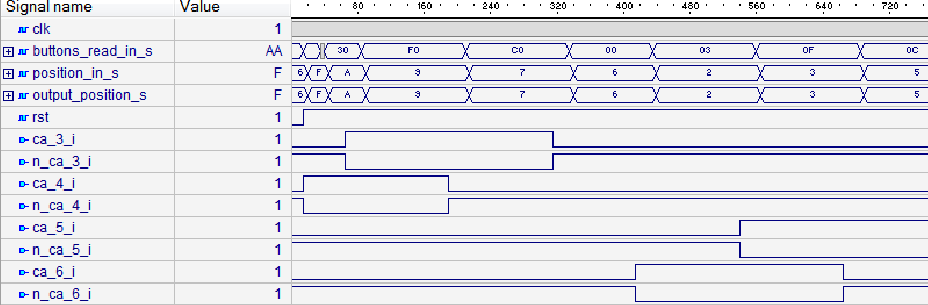
\includegraphics[width=\textwidth]{images/Position-sim.pdf}}
\caption{Simulation of the Position Acquisition module for each input combination (requirement: Input R2)}
\label{position_sim}
\end{figure}


In addition to the simulation results for each module, value checking was also applied to the design using UVVM to ensure the correct value is calculated. The results of the UVVM checking for the Position sub-module are shown in Figure \ref{uvvm_results}. The textual output corresponds to the same simulation displayed for the Position sub-module. As the simulation progresses, the values at any time along the simulation can be verified and the results are summarised at the end of the simulation. If a value is found to be incorrect for any of the checks then it is flagged and the actual value is presented which aids debugging. The textual response for this module shows each of the stages of the verification plan. The module was swept through from Position one, through each intermediate position, to Position two. Example UVVM code for a single check, which corresponds to a line in the summary table, is shown in Appendix Item \ref{UVVM_Position_Code}. The code shows the stimulation, value checking and timing verification that are applied using UVVM methods. This pattern was applied for each position in the simulation.
The results were also checked for invalid position inputs. Timing verification, ensuring the filter is working as expected, is also performed and the results are presented.

\begin{figure}[h]
\centering
\fbox{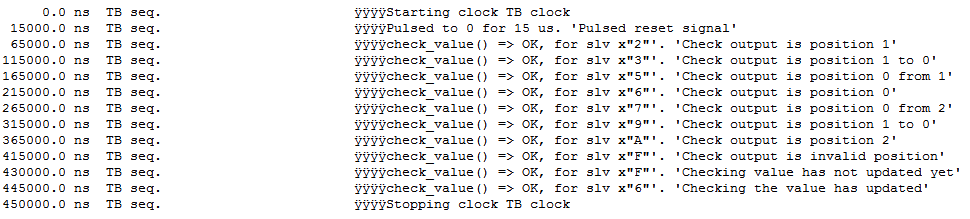
\includegraphics[width=\textwidth]{images/uvvm_results.png}}
\caption{UVVM verification output example for the Position module simulation}
\label{uvvm_results}
\end{figure}

The other sub-modules in the Input Processing module were also simulated and verified. The same process that was applied to the Position Acquisition sub-module was applied in the verification of Command interpretation. Each of the valid commands were swept through and the output of the Command sub-module was monitored and verified using UVVM. The other sub-modules in the Input module relate to the control of direction and timings of the movement. For the verification of the sub-module for requirement Input R3, responsible for the decision making in terms of movement and direction, each combination of command input and position was provided and the expected result was analysed. The response included raising a flag to indicate that movement is necessary and providing the correct direction of movement. The sub-module which was responsible for the timing control of the motor control process was verified using UVVM timing functions. The UVVM functions wait for a given event and then can verify that the timing of that event matches the required time. Alternatively, they can wait a given time and verify that the value is correct at that time. This was applied over several of the application cases including a successful movement first time, a successful movement upon a retry and an unsuccessful movement in order to verify that the response of the design matched the specification for each case.

\subsection{ADC Verification}

In order to verify the ADC, an analogue input must be modelled by the simulation. This required creating a model of the RC input stage. The ADC, which was obtained from Lattice, came with a verification file. In this verification file, integrators are used to simulate the RC input stage and the comparitor at the input of the FPGA. A saw-tooth input was generated in this simulation in order to verify the response of the ADC. 

\begin{figure}[h]
\centering
\fbox{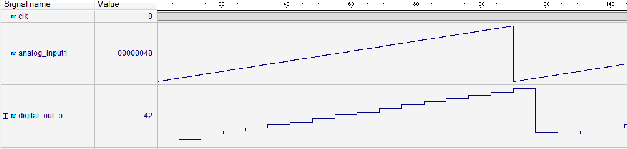
\includegraphics[width=\textwidth]{images/ADC-sim.pdf}}
\caption{ADC simulated response to a saw-tooth waveform (requirements: ADC R1 and ADC R2)}
\label{adc_sim}
\end{figure}

The simulation results in Figure \ref{adc_sim} show the response of the ADC to this saw-tooth input. The response can be seen to follow the saw-tooth ramp closely. When the saw-tooth resets and falls from the maximum value to the minimum value, the ADC can be seen to follow the value with the behaviour of an averager as it falls through an intermediate value before increasing again. UVVM was applied to this simulation throughout to ensure the value is within a one-bit tolerance of the input value for each reading. The ADC produces periodic values and holds the value until it has calculated the next one so the response is more stepped than the simulated analogue input. 

\subsection{PWM Regulation Verification}
\label{regulation-results}
In order to test the PWM regulation scheme, the regulation loop, shown in Figure \ref{motor_control_loop}, must be simulated. This includes modelling the motor in order to verify the response to an actual motor. Under normal switching conditions, regulation of motor current is not needed as the current is consistently below 1.5A. The regulation process operates when the motor is stalled or blocked. In order to verify the response of the motor to these conditions, a stalled motor has to be modelled in the simulation. It is difficult to accurately simulate the actual response of an analogue motor controlled by a VHDL design\cite{Dubey}. Matlab can be used for mixed-signal simulations\cite{Dubey}, however; it will not be adopted by this project as a simplified model of the stalled motor was sufficient for regulation testing and fine-tuning. The model consisted of a VIR calculation based on the PWM signal (V), the resistance of the motor (R) and the calculated resulting current (I) which was fed back into the regulation unit. UVVM was used to perform the calculations required to model the motor and provide the new stimulus.

\begin{figure}[h]
\centering
\fbox{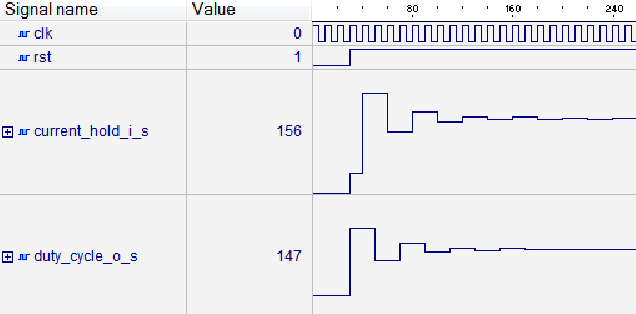
\includegraphics[width=0.65\textwidth]{images/Regulation-sim.pdf}}
\caption{PWM regulation simulation of a stalled motor modelled in UVVM (requirement: PWM R2)}
\label{regulation_sim}
\end{figure}

The simulation results for the PWM Regulation module are shown in Figure \ref{regulation_sim}. The diagram shows the response of the duty-cycle to the measured current for the regulation process. The regulation module aims to keep the current value at a nominal value. It achieves this by adjusting the PWM duty-cycle, which drives the motor, based on the measured current from the ADC. In this simulation, the current is calculated from the effect of the duty-cycle value on a fixed resistance. It can be seen in the diagram that the initial value of current is measured to be too low, compared to the regulation value. In response to this, the regulation module increases the duty-cycle. The response of the motor model produces a current which is now above the regulation value, the duty-cycle is then reduced accordingly. This process repeats until the values stabilise and the regulation current is achieved. In this example, the regulation current was set to the ADC value of 155 and the value alternates between 155 and 156. The response, which can be seen in this simulation, is typical to that of a proportional controller. UVVM checking was also applied to ensure that each of the PWM Regulation requirements were met by the design. The additional sub-modules which were responsible for providing the correct control signals to the regulation process were generated using UVVM for this simulation and were verified separately.

The PWM module design contains a number of state machines in order to generate the required control signals; each of which needs to be fully verified. OSVVM was applied to each of them to ensure that each machine reaches each possible state during the simulation. The application of state transition monitors provides instant and automatic feedback. An example response from OSVVM, applied to the PWM control state machine, can be seen in Figure \ref{osvvm_results}. The response shows a calculation of the state coverage. In this case the coverage is 100\%. The results for each transition are printed in the response. This includes a count of the number of transitions between states throughout the simulation for each mapping and a flag indicating that the transition occurred. The OSVVM code which set up these transition bins can be seen in Appendix Item \ref{OSVVM_Motor_Bins}. This instant feedback ensures that the test plan has been completed by ensuring that all states are realised in the simulation. OSVVM was applied to all state machines in the design and identified cases which were not originally covered in the test plan. The test plan was modified in iterative cycles and the final test-suite provided 100\% state coverage.

\begin{figure}[h]
\centering
\fbox{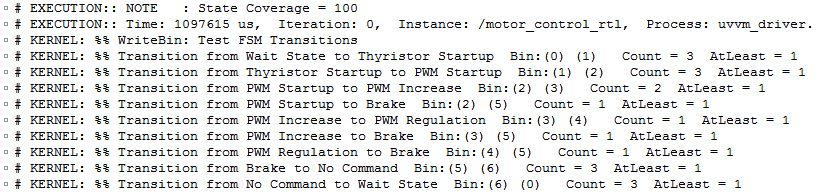
\includegraphics[width=\textwidth]{images/osvvm_results.png}}
\caption{OSVVM state coverage results for the PWM control state machine (requirement: PWM R1)}
\label{osvvm_results}
\end{figure}

\subsection{Motor Driving Verification}

The Motor Driving module is required to drive the correct IGBT and Thyristor combinations based on control signals provided by other modules. The behavioural response to each of the control signal combinations must be verified against the specification to ensure that it is not possible for invalid combinations of IGBTs and Thyristors to be driven. The output control signal combinations from the Input Processing and PWM Regulation modules were generated using UVVM and the response was verified using the same methodology.

The simulation results for the IGBTs during a motor movement can be seen in Figure \ref{igbt_sim}. The control signals which were created as part of the motor control process were simulated. The conditions for each respective IGBT being driven are checked by the simulation. The PWM signal, produced by the simulation to model the accurate behaviour of the system, was sent to the IGBT for the correct direction indicated. For example, the simulation shows the completion of one of the sub-module requirements for the IGBT: if the IGBT is enabled (en\_db\_o\_s is set to 1) then the PWM generated by the regulation process (pwm\_i\_s) should be passed directly to the IGBT for the given direction (pwm\_db\_o\_s). Each of the combinations of the control signals was verified using UVVM. The braking phase can also be seen in the diagram where the brake\_i\_s signal is driven. For this phase, which is required to stop the motor, each of the IGBTs are driven. 

\begin{figure}[h]
\centering
\fbox{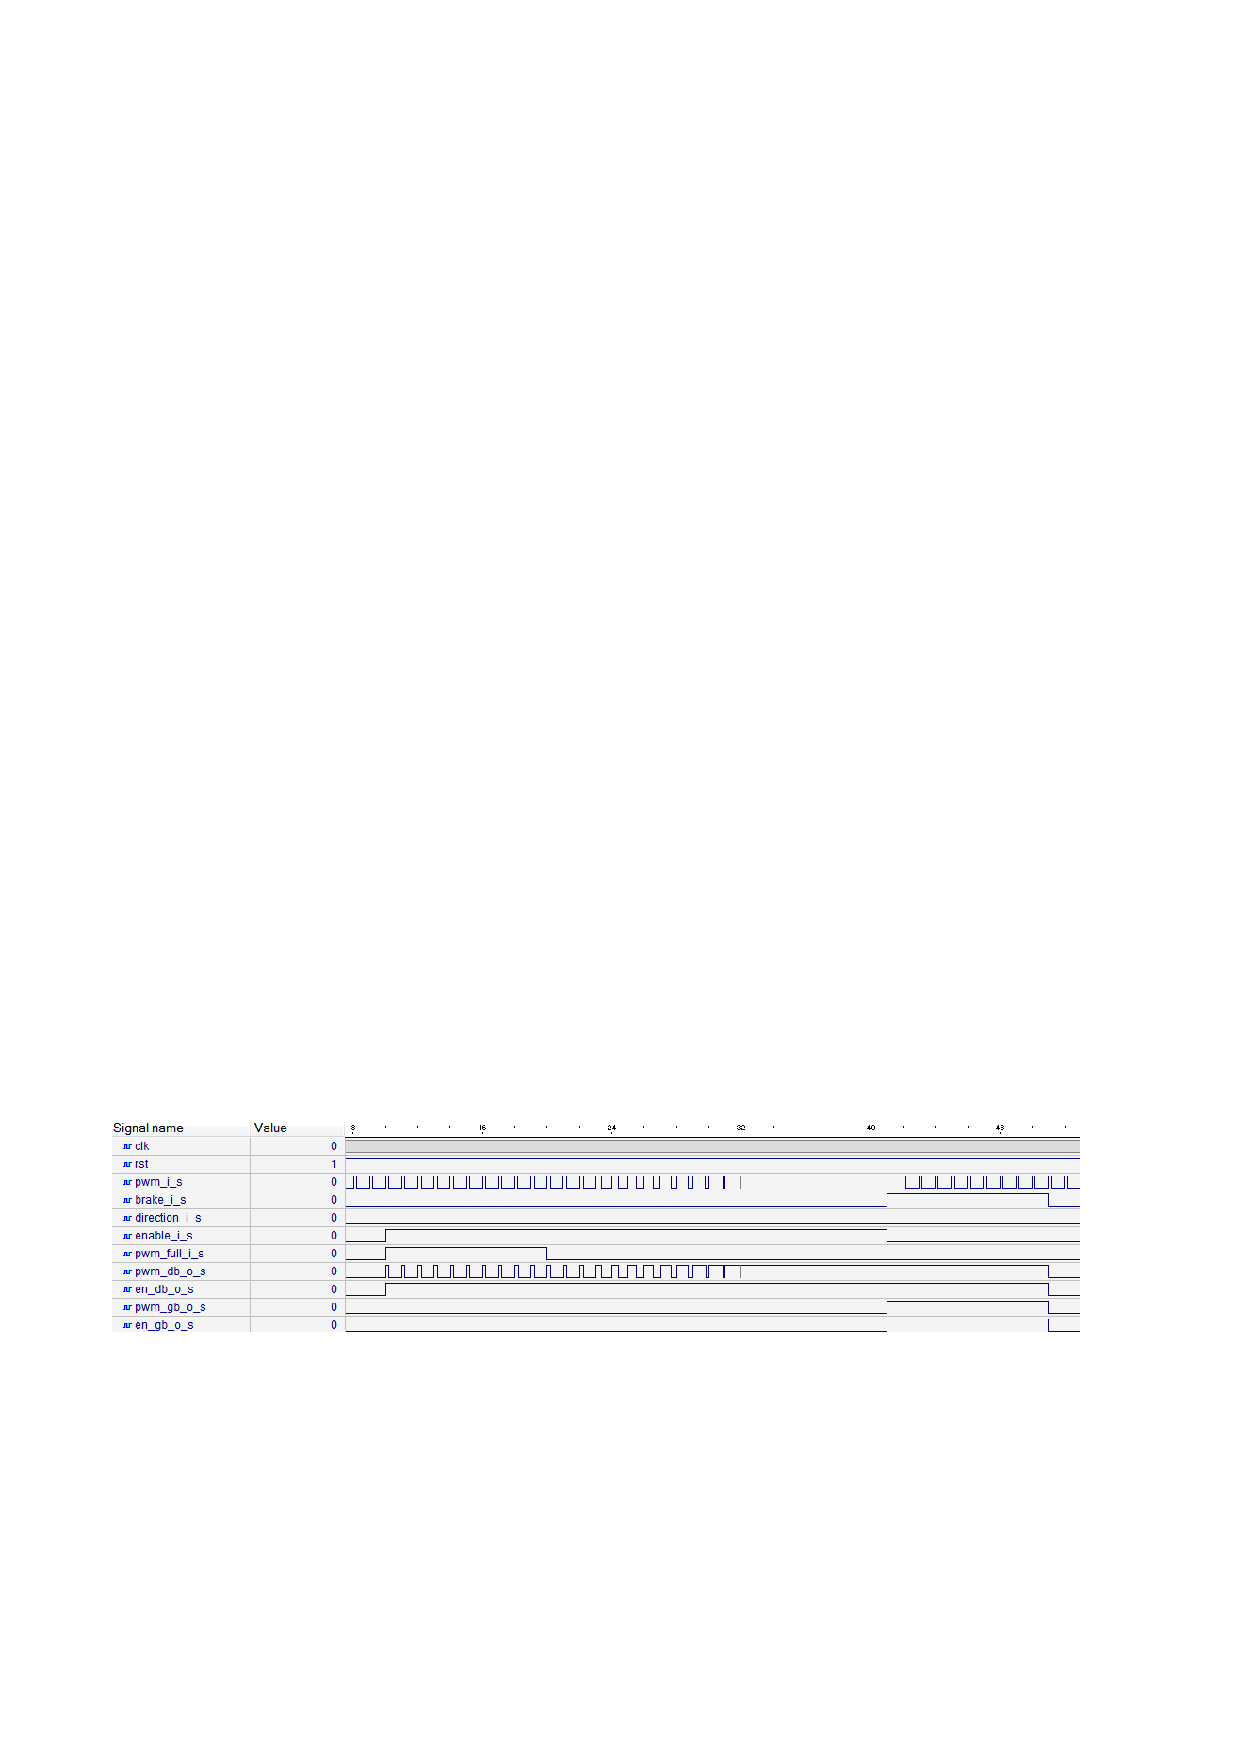
\includegraphics[width=\textwidth]{images/IGBT-sim.pdf}}
\caption{Simulation of the IGBT throughout the simulated motor control process (requirement: Drive R1)}
\label{igbt_sim}
\end{figure}



\section{Further Verification}
Behavioural verification of each module of the design was performed using UVVM; however, there were some verification activities, required by SIL, which were not completed in simulation for this project. These activities include system-level verification which is related to the interaction between different modules. Additionally, gate-level simulations which give insight into the synthesised timings of the design were not performed using UVVM.

\subsection{System Verification}

System behaviour can be validated by verifying multiple modules and their interactions. For this project, this process was done on the physical prototype. As described in the prototype creation Section \ref{prototyping-strategy}, the modules were tested on the PCB by incrementally integrating sub-modules. By verifying this using UVVM the benefits of automatic verification could be realised. This would provide the design with a more comprehensive test-suite which verifies each level of the module. Any number of modules can be incorporated into a simulation for UVVM. This could scale up to the entire design where the requirements of the entire end-to-end system can be validated. This is the final process of the V-model. 

\subsection{Gate-level Simulations}

Gate-level simulations can be performed on the synthesised design. This allows accurate modelling of the timing behaviour of the system. Where register-transfer-level simulations provide behavioural verification, gate-level simulations provide insights into true time-based behaviour. Behavioural verification was the focus for this project. The prototyping activities on the physical PCB gave insight into and verification of the general timing behaviour of the system; however, by applying verification methodologies to the gate-level design, the timing verification of the design could be realised. 



%Others:
%How OSVVM is being used for this
%SIL requires 100\% coverage
%How UVVM is being used for stimulation
%Simplifies the verification code and makes it easier to read/understand
%How UVVM is being used for value checking
%Automates the validation process (prevents manual inspection of simulation results, reduces the verification time)
%Using UVVM for timing analysis
%Essential for the verification of time-based requirements (real-time systems) like motor control (find source)
%Automates the validation process



% realtime digital simulator for motor drives? \cite{Zhang}
% VHDL-AMS (mixed signal) \cite{Acero}


\section{Verification Conclusion}

Verification methodologies were systematically applied to directly verify the project requirements. UVVM was used to verify the functional behaviour of each modules in the design to ensure that they matched the specification. The automated value checking of UVVM reduced the need for manual inspection of simulation graphs and allowed for instant verification feedback. OSVVM was applied to each of the state machines in the system to ensure that they were all fully covered by the simulation. OSVVM was applied to map each of the transitions of state machines in the design to provide coverage metrics for the simulations. The verification of the design validated all of the project requirements with a 100\% state coverage. System and gate-level simulations were applied on the physical prototype of the project. By applying UVVM to these verification areas, the benefits of methodologies could be realised for integration and timing behaviour. All of the modules in the design were verified individually and each of the requirements were directly mapped into the verification plan providing a comprehensive coverage of validation of the requirements of the design.  